\documentclass[aspectratio=169]{beamer}
\usetheme{Madrid}

\usepackage{tikz}
\usetikzlibrary{arrows.meta, positioning, calc}
\usepackage{graphicx}
\usepackage[utf8]{inputenc}
\usepackage{hyperref}
\usepackage{listings}

\begin{document}

\title{Introduction to neural networks}   
\subtitle{Training aspects} 
\author[J.I. Vasquez]{\textbf{Juan Irving Vásquez} \\jivg.org}
\date{\today \copyright}
\institute[jivg.org]{Centro de Innovación y Desarrollo Tecnológico en Cómputo \\ Instituto Politécnico Nacional}
% logo of my university
\titlegraphic{
\includegraphics[width=2cm]{ipn-cidetec}}
\frame{\titlepage} 


\frame{
	\frametitle{Contents}
	\tableofcontents
}


\AtBeginSection[] { \begin{frame} \frametitle{Roadmap} \tableofcontents[currentsection] \end{frame} }


%%%%%%%%%%%%%%%%%%%%%%%%%%%%%%%%%%%%%%%%%%%%%%%%%%%%%%%%


\section{Performance measurement}


\frame{
	\frametitle{Performance measurement}
	\begin{itemize}
		\item The central challenge in machine learning is that we must perform well on new,
		\textbf{previously unseen} inputs. 
\begin{center}
	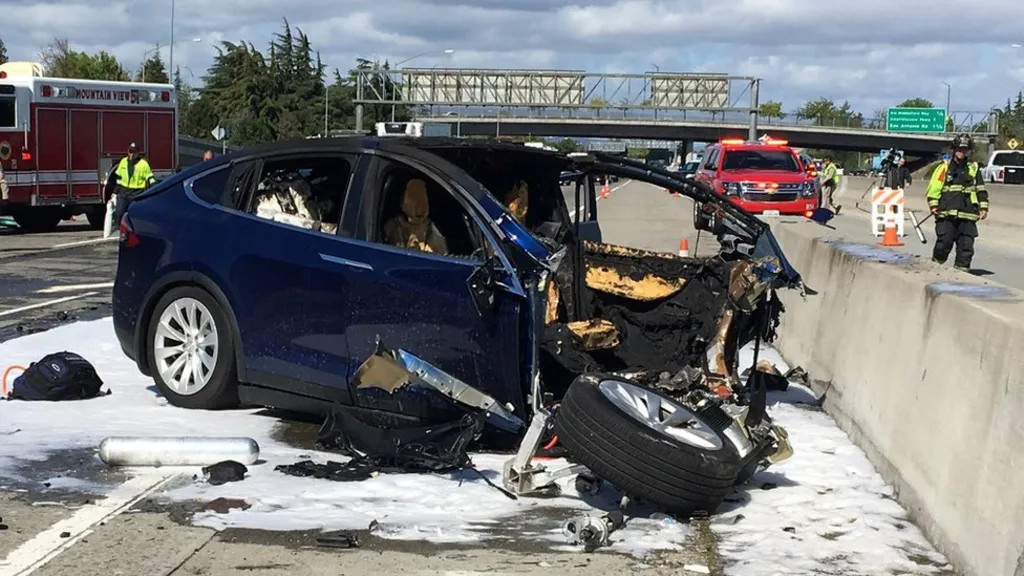
\includegraphics[height=0.4\textheight]{_100644437_hi045823502}\footnote{\tiny https://www.bbc.com/news/world-us-canada-43604440}
	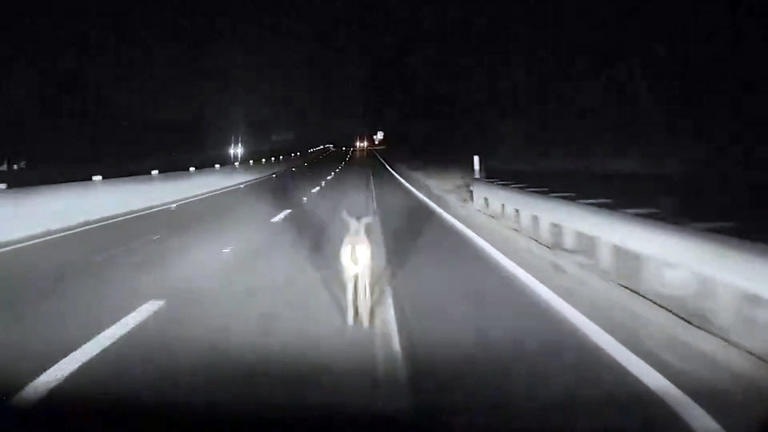
\includegraphics[height=0.4\textheight]{AA1tdRq6.jpeg}\footnote{\tiny https://www.formacar.com/en/tesla--63631--article}
\end{center}
		\item The ability to perform well on previously unobserved inputs is called \textbf{generalization}.
		\begin{itemize}
			\item Dataset split
			\item Metric
			\item Significance
		\end{itemize}
	\end{itemize}
}


\frame{
	\frametitle{Performance measurement}
	We will introduce a validation step and a test in order to measure generalization.
	\begin{figure}
		\centering
		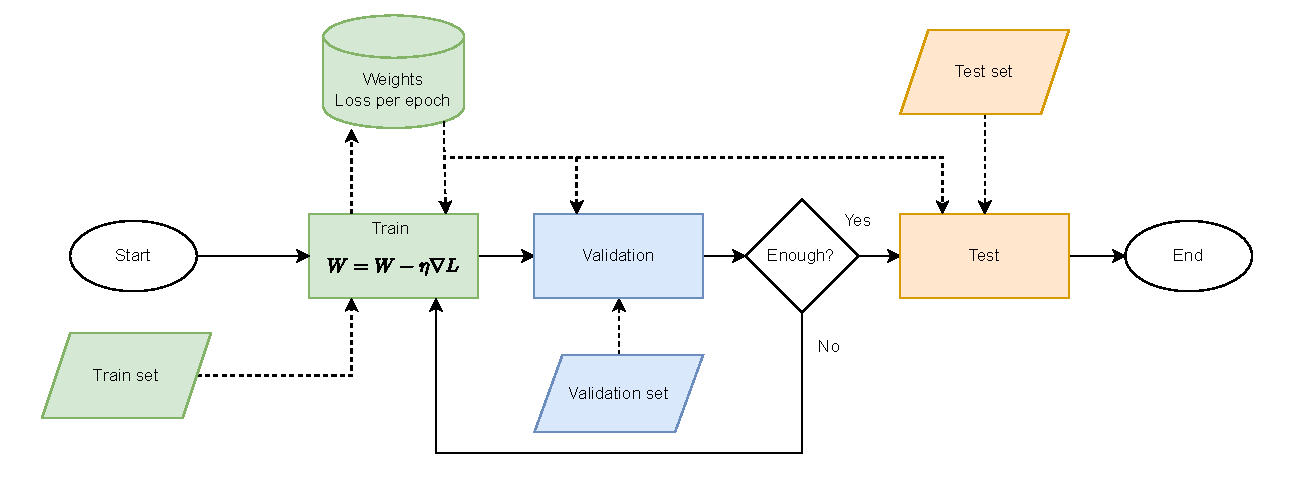
\includegraphics[height=0.55\textheight]{train_and_test_color}
		\caption{Train and test workflow}
		\label{fig:trainandtest}
	\end{figure}
}


\section{Dataset split}


\frame{
\frametitle{Dataset split}
\begin{figure}
	\centering
	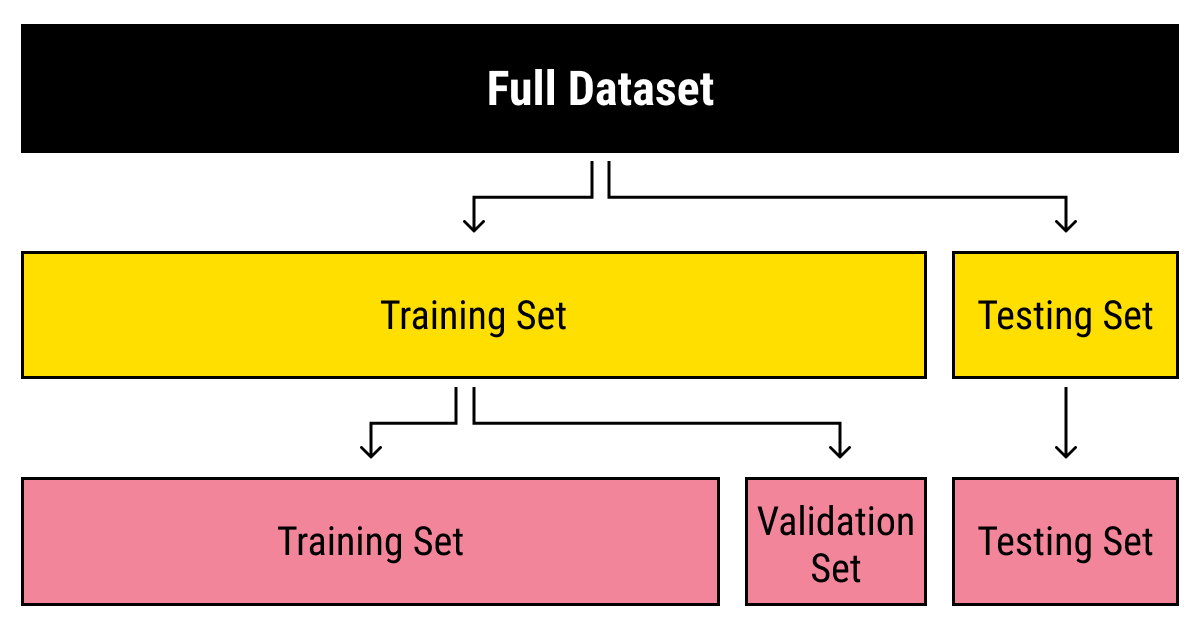
\includegraphics[height=0.7\textheight]{splitting_data}
	\caption{Dataset split [HJC]}
	\label{fig:splittingdata}
\end{figure}
}

\frame{
	\frametitle{Training and validation set split}
	\framesubtitle{N-fold validation}
	\begin{itemize}
		\item Lets suppose a dataset, $X_\Omega = \{x_1, \dots, x_m\}$,  with positive examples
		\item We could use a subset of our set of observations as an
		estimate of the performance 
		$$X = {x_1,\dots, x_n}$$
		$$X' = {x_{n+1},\dots,x_{m}}$$, $X$ is the \textbf{training set} and $X'$ is usually called the \textbf{validation set} [Smola].
		\item Typically, one uses about 80\% of the training data for training and
		20\% for validation [GoodFellow].
	\end{itemize}
}


\section{Performance metrics}


\frame{
	\frametitle{Performance metrics}
	Common measurements for categorical outputs
	\begin{itemize}
		\item Accuracy
		\item Precision
		\item Recall
		\item F1 score
	\end{itemize}
}



\frame{
	\frametitle{Confusion matrix}
		\begin{itemize}
			\item Computation:
			\begin{table}
						\begin{tabular}{|c|c|c|}
					\hline
					Ground truth& \textbf{Positive Prediction} & \textbf{Negative Prediction} \\ \hline
					\textbf{Positive Class} & TP & FN \\ \hline
					\textbf{Negative Class} & FP & TN \\ \hline
				\end{tabular}
				\caption{Confusion matrix}
			\end{table}
			\item TP + FN sums 100 \% of the positive class
			\item FP + TN sums 100 \% of the negative class
		\end{itemize}
}


\frame{
	\frametitle{Example}
	%\framesubtitle{Dataset}
	\begin{figure}
		\centering
		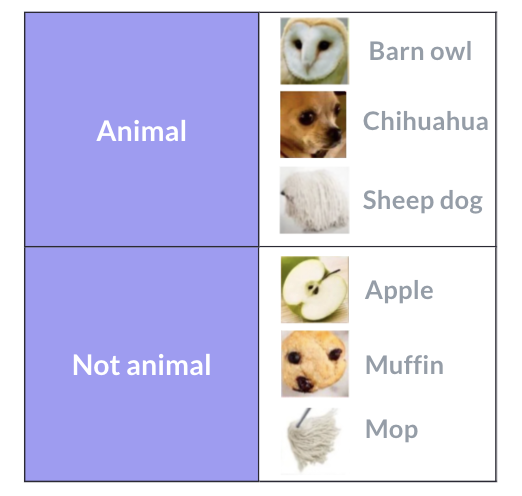
\includegraphics[height=0.7\textheight]{ds}
		\caption{Dataset of animals and no animals. \footnote{https://www.labelf.ai/blog/what-is-accuracy-precision-recall-and-f1-score}}
		\label{fig:ds}
	\end{figure}
}


\begin{frame}
	\frametitle{Prediction concepts}
	\framesubtitle{For binary classes\footnote{Consider the class 'animal' as the positive class.}}
	\centering
	\begin{tabular}{|c|c|c|}
		\hline
		Network input & Prediction & Concept \\
		\hline
		
\includegraphics[width=0.09\textwidth]{chihuahua} & 'animal' & true positive \\
		
\includegraphics[width=0.09\textwidth]{chihuahua} & 'not animal' & false negative \\
		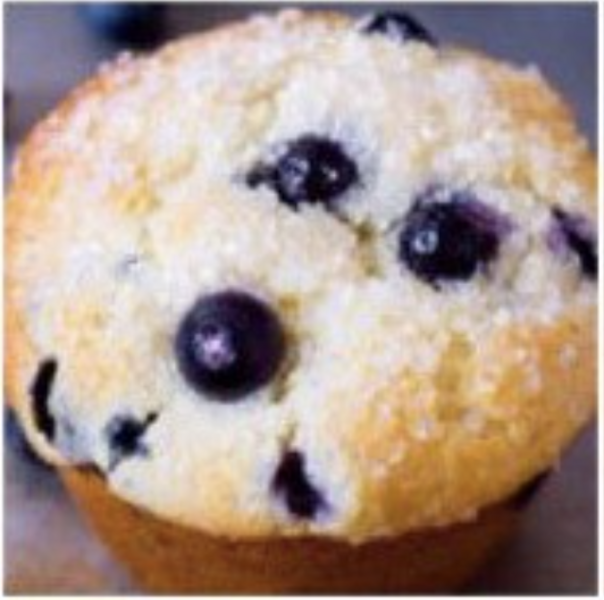
\includegraphics[width=0.09\textwidth]{muffin} & 'animal' & false positive \\
		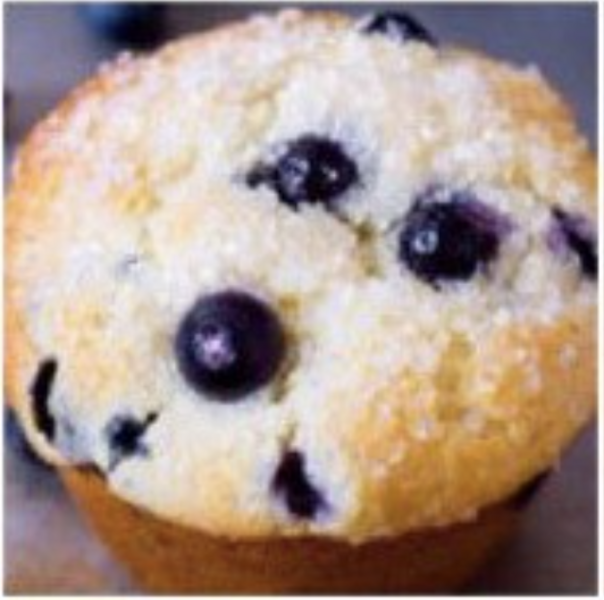
\includegraphics[width=0.09\textwidth]{muffin} & 'not animal' & true negative \\
		\hline
	\end{tabular}
\end{frame}


\frame{
	\frametitle{Confusion matrix}
\begin{figure}
	\centering
	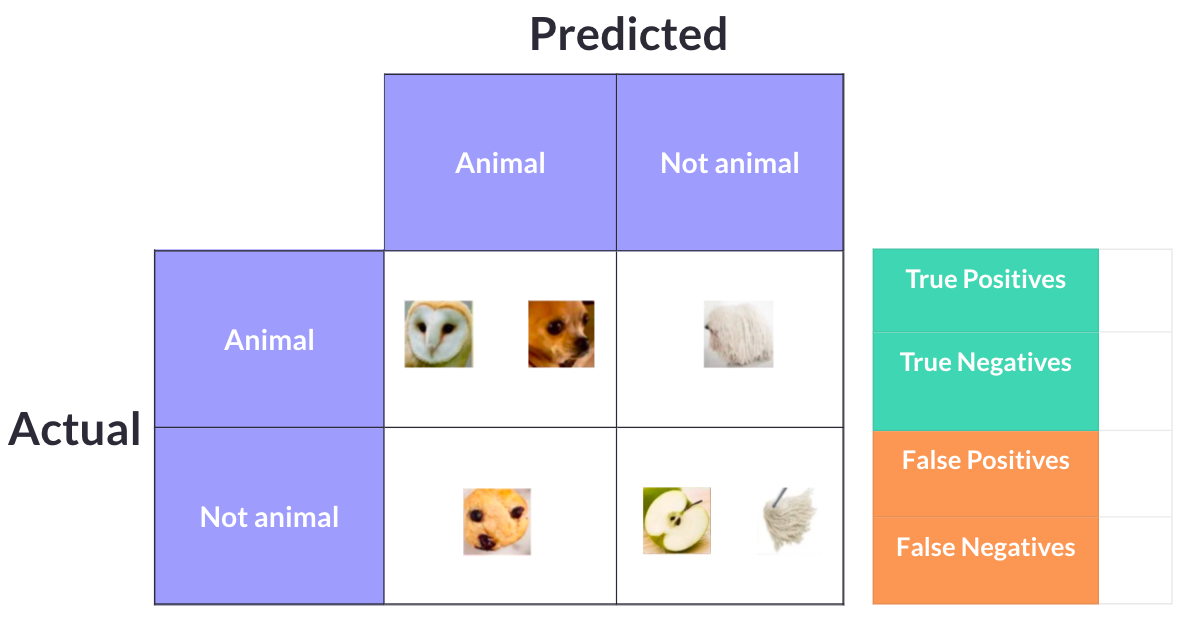
\includegraphics[height=0.75\textheight]{mc1}
	\caption{Confusion matrix example.}
	\label{fig:mc1}
\end{figure}
}

\frame{
	\frametitle{Confusion matrix}
	\begin{figure}
		\centering
		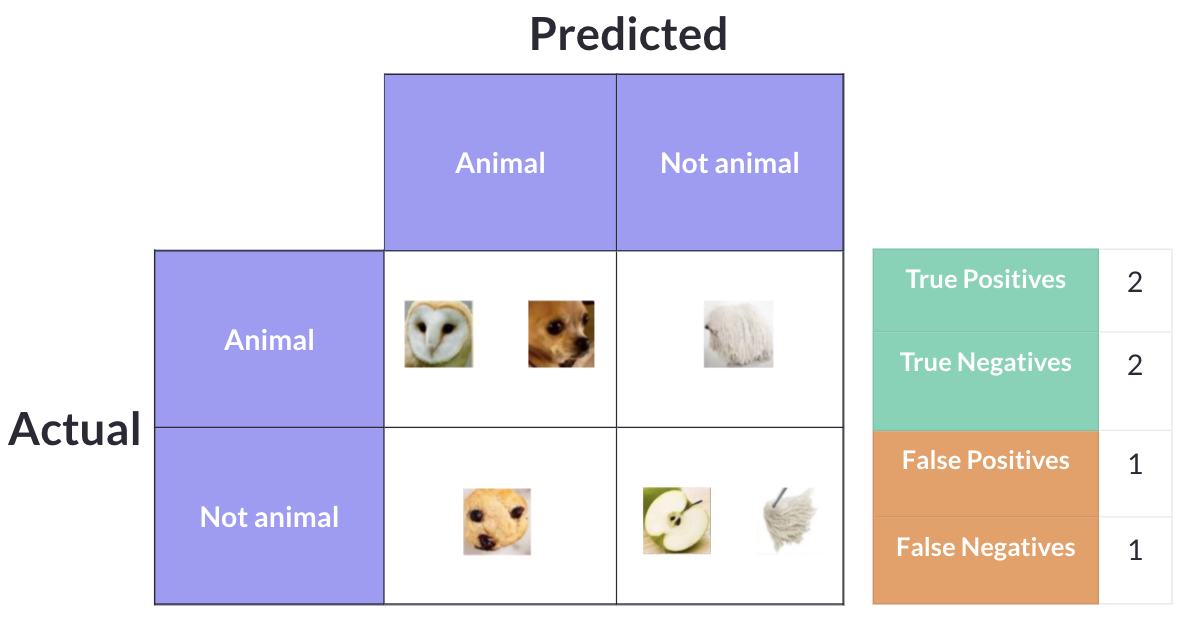
\includegraphics[height=0.75\textheight]{mc2}
		\caption{Confusion matrix example.}
		\label{fig:mc1}
	\end{figure}
}

\frame{
	\frametitle{Performance metrics}
	\framesubtitle{Accuracy}
	
	\begin{equation}
		\text{Accuracy} = \frac{TP + TN}{TP + TN + FP + FN}
	\end{equation}
	
	TP represents true positives, TN true negatives, FP false positives, and FN false negatives.
}



\frame{
	\frametitle{Performance metrics}
	\framesubtitle{Precision}
	
	\begin{equation}
		\text{Precision} = \frac{TP}{TP + FP}
	\end{equation}
	
	In this formula, TP represents true positives and FP false positives. This metric measures the proportion of positive identifications that were actually correct.
}



\frame{
	\frametitle{Performance metrics}
	\framesubtitle{Recall}
	\begin{equation}
		\text{Recall} = \frac{TP}{TP + FN}
	\end{equation}
	TP represents true positives and FN false negatives. Recall measures the model’s ability to find all relevant positive instances in the dataset.
}



\frame{
	\frametitle{Performance metrics}
	\framesubtitle{F1-score}
	
	The F1-score, which is the harmonic mean of precision and recall, can be expressed as:
	
	\begin{equation}
		F1 = 2 \times \frac{\text{Precision} \times \text{Recall}}{\text{Precision} + \text{Recall}}
	\end{equation}
	
	Thus, the F1-score combines both precision and recall into a single metric that accounts for both false positives and false negatives. It is especially useful in situations where the balance between precision and recall is critical.
}

\frame{
	\frametitle{Significance}
	\begin{center}
		
\includegraphics[height=0.85\textheight]{./FB_IMG_1679059875964}
	\end{center}
}


\frame{
	\frametitle{Significance}
	\begin{center}
		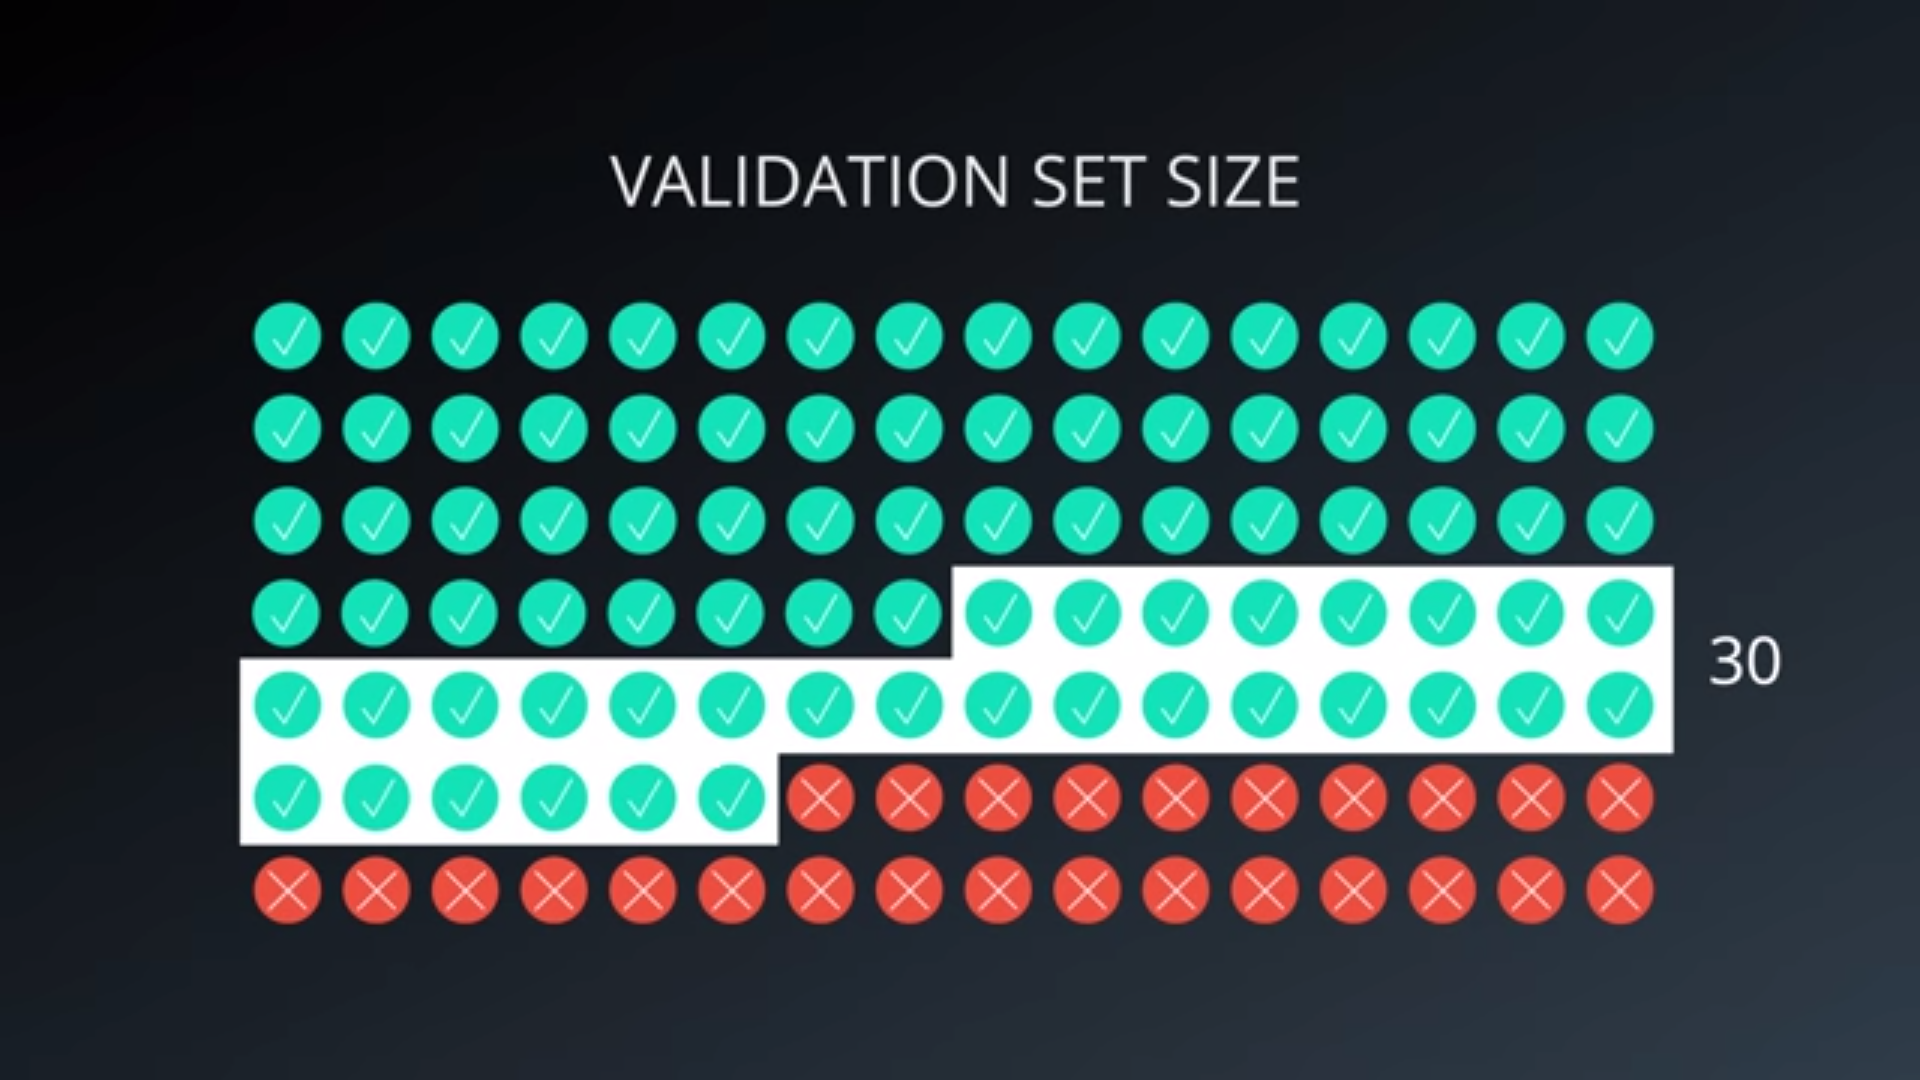
\includegraphics[width=0.8\linewidth]{./significance}
	\end{center}
}

\begin{frame}{Statistical Significance \& Model Evaluation}
	\begin{block}{Definition}
		A result is statistically significant if the probability of it occurring by chance is very low, typically defined by a threshold $\alpha$ (e.g., $0.05$).
	\end{block}
	
	\vspace{0.3cm}
	
	\textbf{Core Concepts:}
	\begin{itemize}
		\item \textbf{Null Hypothesis ($H_0$):} No real difference between models.
		\item \textbf{p-value:} $P(\text{Data} | H_0)$. If $p < \alpha$, we reject $H_0$.
	\end{itemize}
	
	\vspace{0.3cm}
	
	\textbf{Application in ML (Model Comparison):}
	To compare error rates $\epsilon_1$ and $\epsilon_2$ using a Z-test:
	
	\begin{equation}
		Z = \frac{|\hat{\epsilon}_1 - \hat{\epsilon}_2|}{\sqrt{\frac{\hat{\epsilon}(1-\hat{\epsilon})}{n_1} + \frac{\hat{\epsilon}(1-\hat{\epsilon})}{n_2}}}
	\end{equation}
	
	\vfill
	\centering
	\textit{Ensures that performance gains are robust and reproducible.}
\end{frame}


\section{Overfitting}


{ 	\usebackgroundtemplate{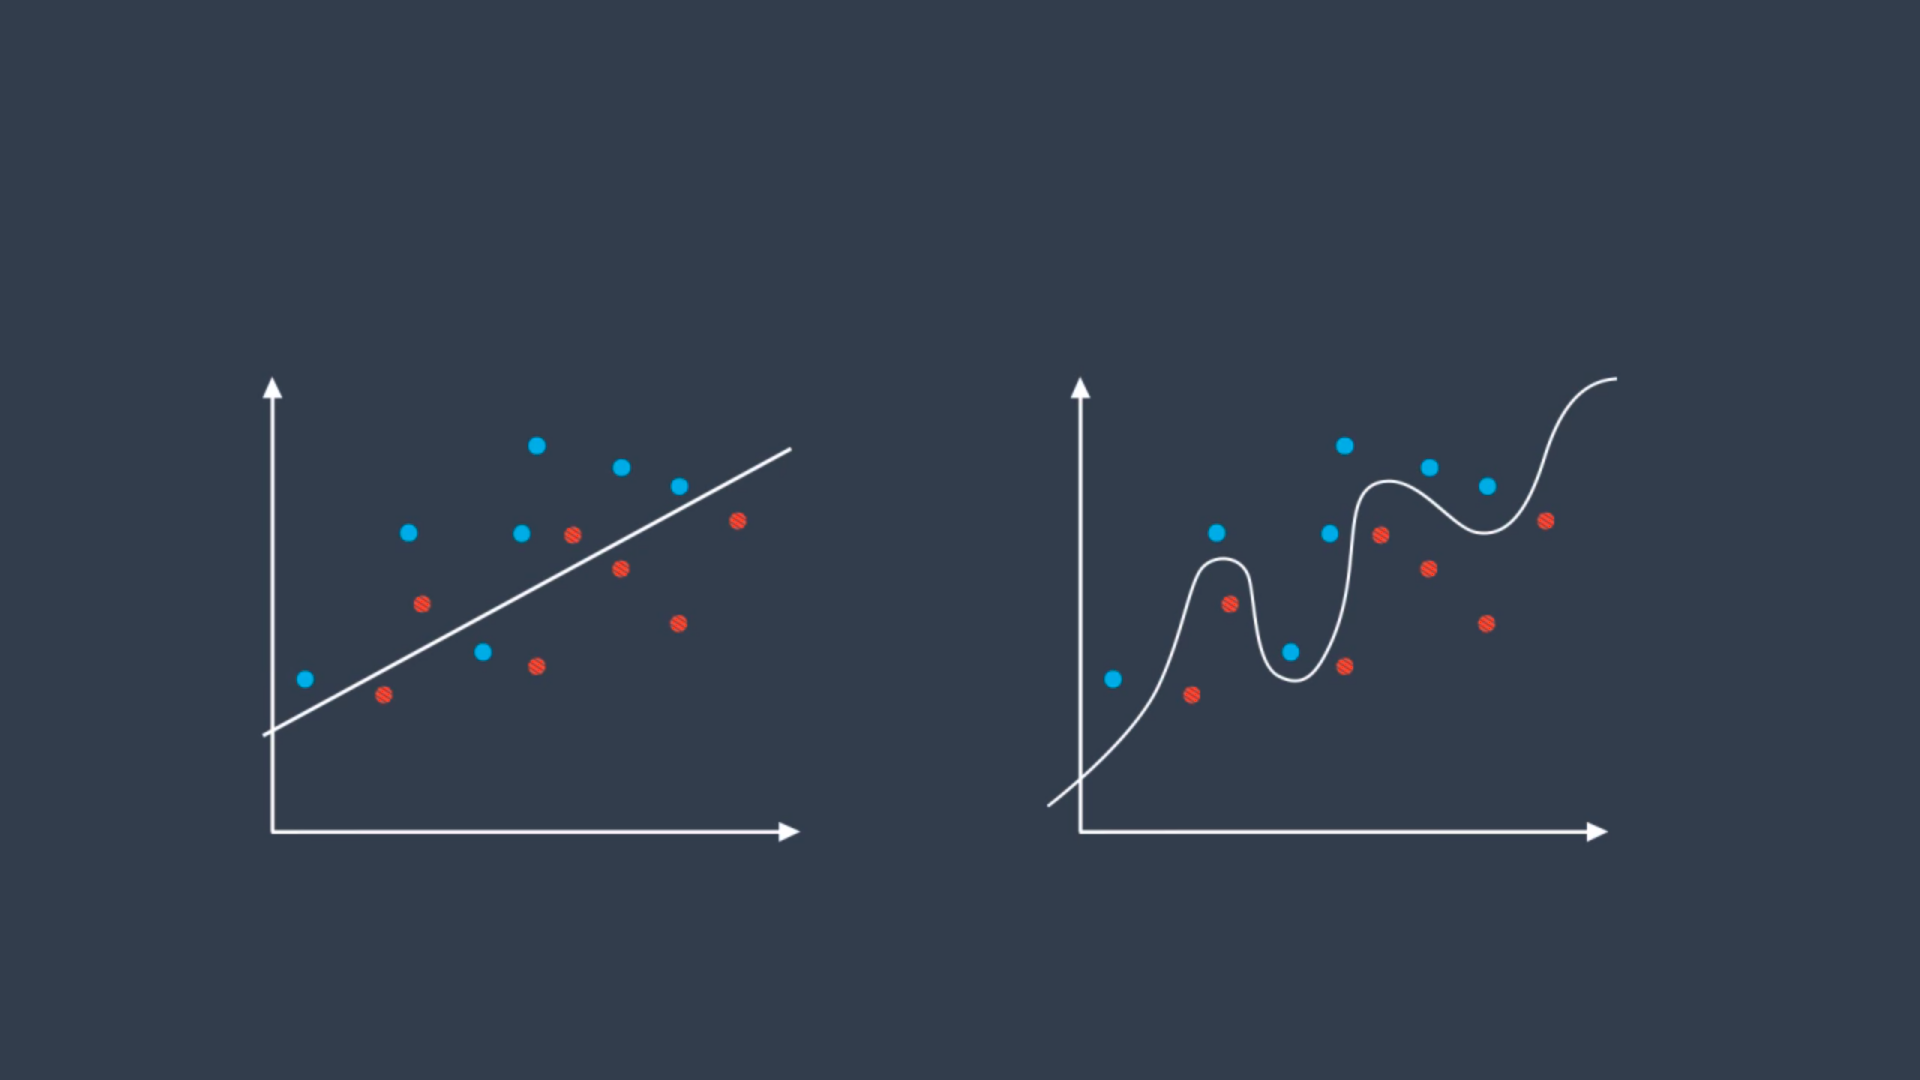
\includegraphics[width=1\paperwidth]{./overfitting1}}%
\frame{
\frametitle{Overfitting problem}
\framesubtitle{Which model is better?}
}
}


{ 	\usebackgroundtemplate{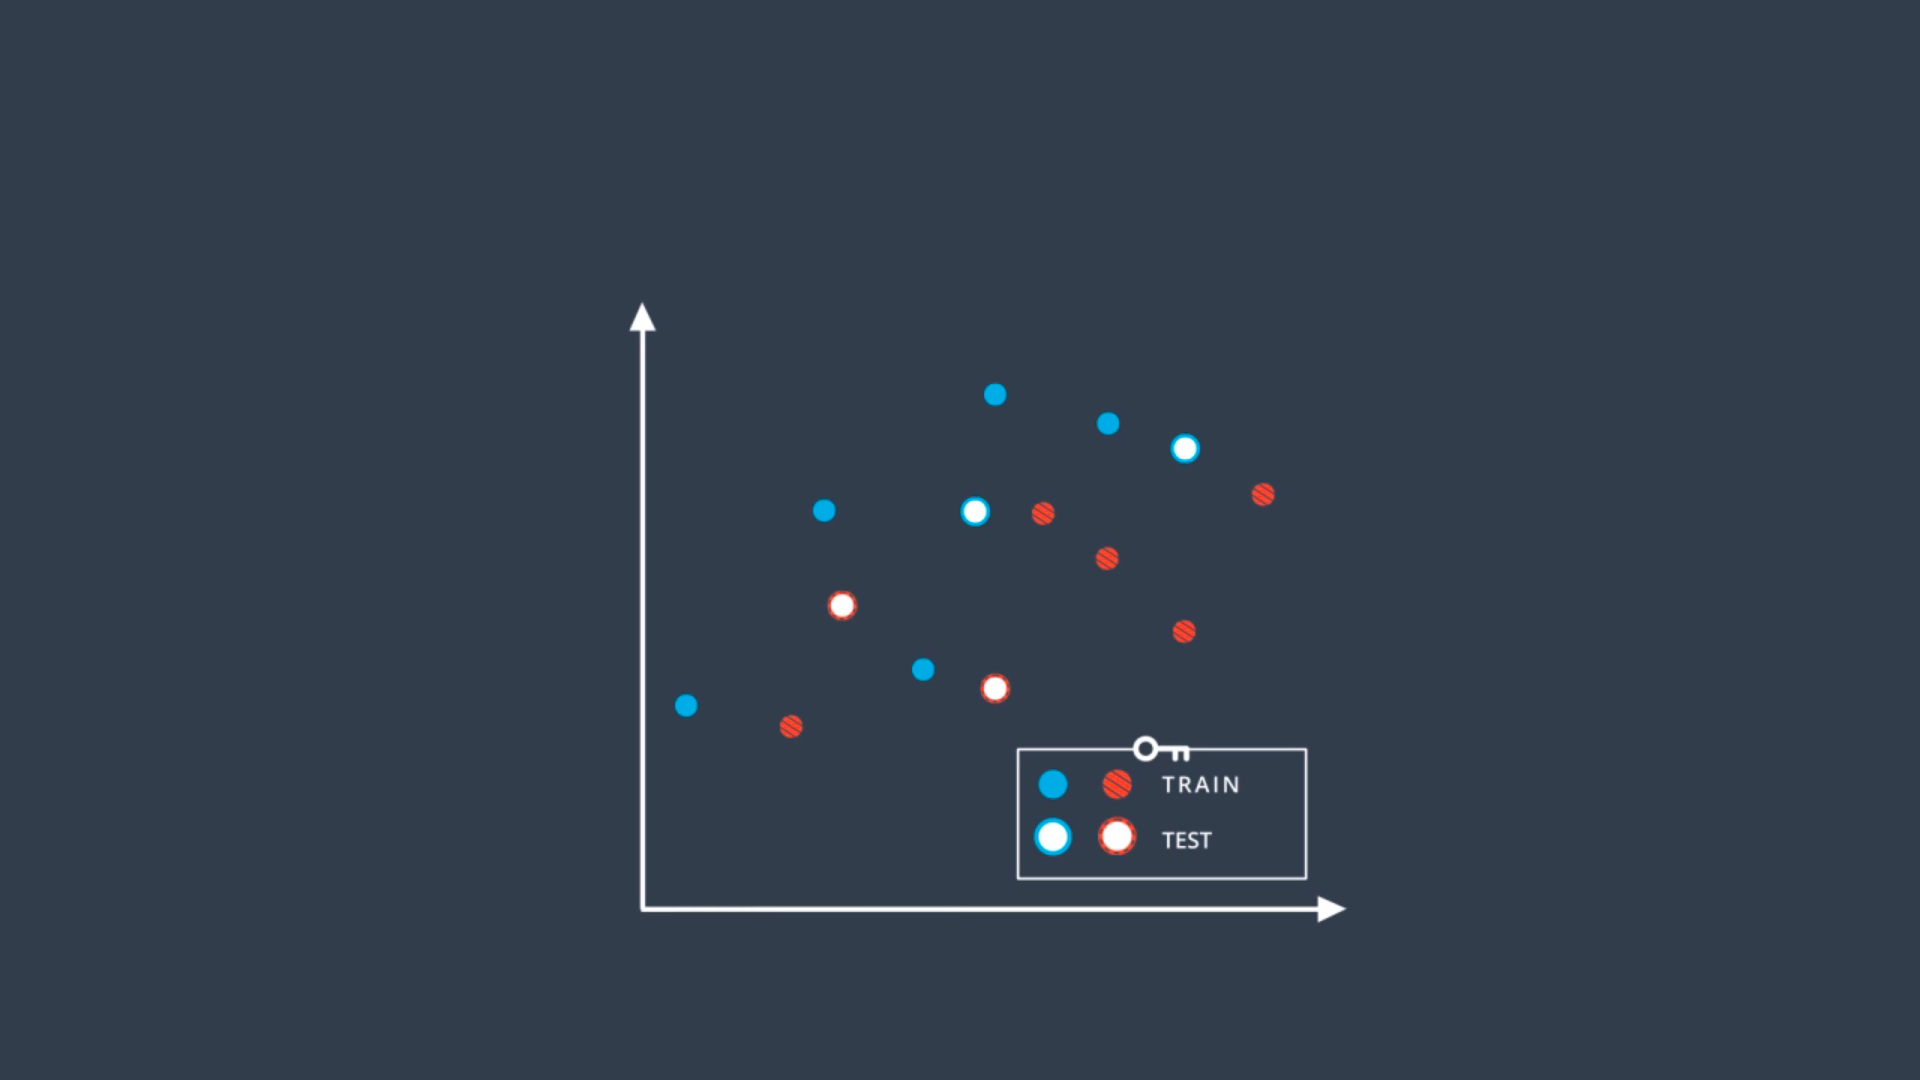
\includegraphics[width=1\paperwidth]{./overfitting2}}%
\frame{
	\frametitle{Overfitting problem}
	\framesubtitle{The importance of testing}
}
}


{ 	\usebackgroundtemplate{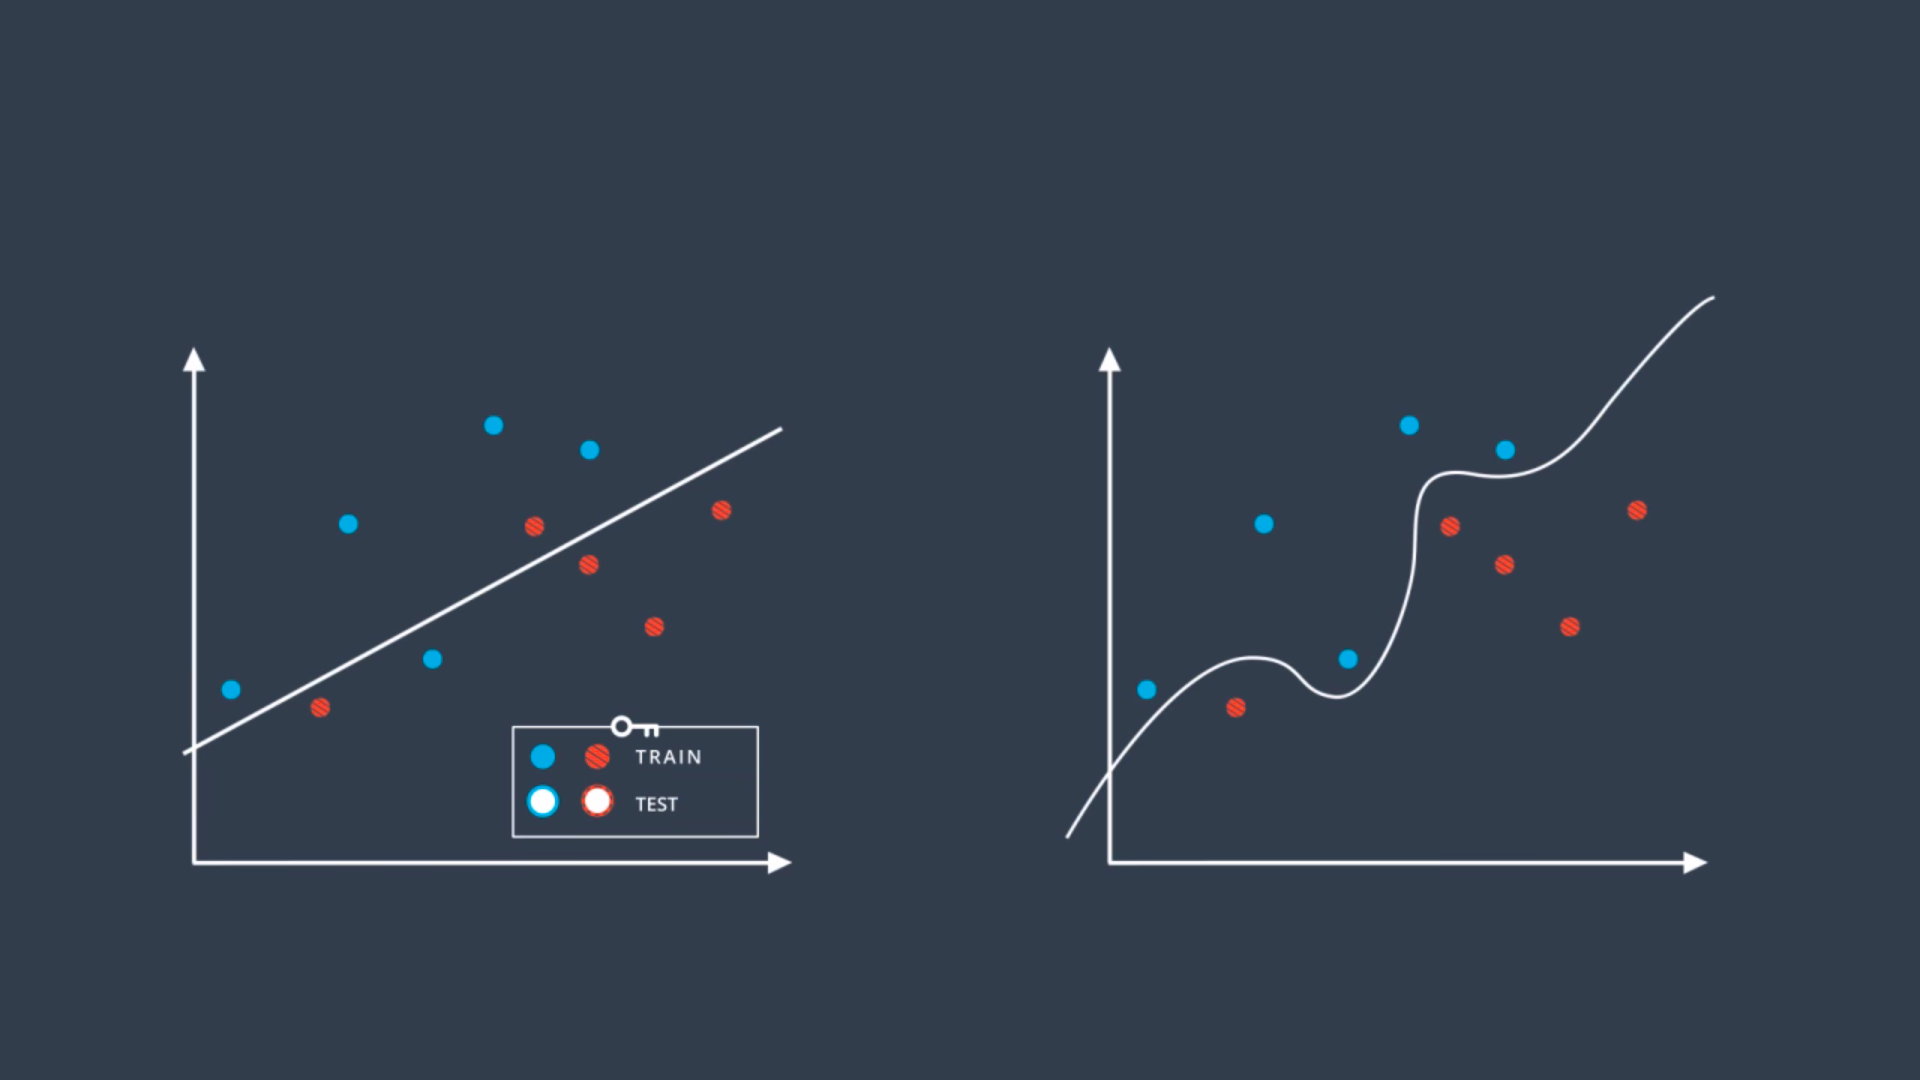
\includegraphics[width=1\paperwidth]{./overfitting3}}%
\frame{
	\frametitle{Overfitting problem}
	\framesubtitle{The importance of testing}
}
}


{ 	\usebackgroundtemplate{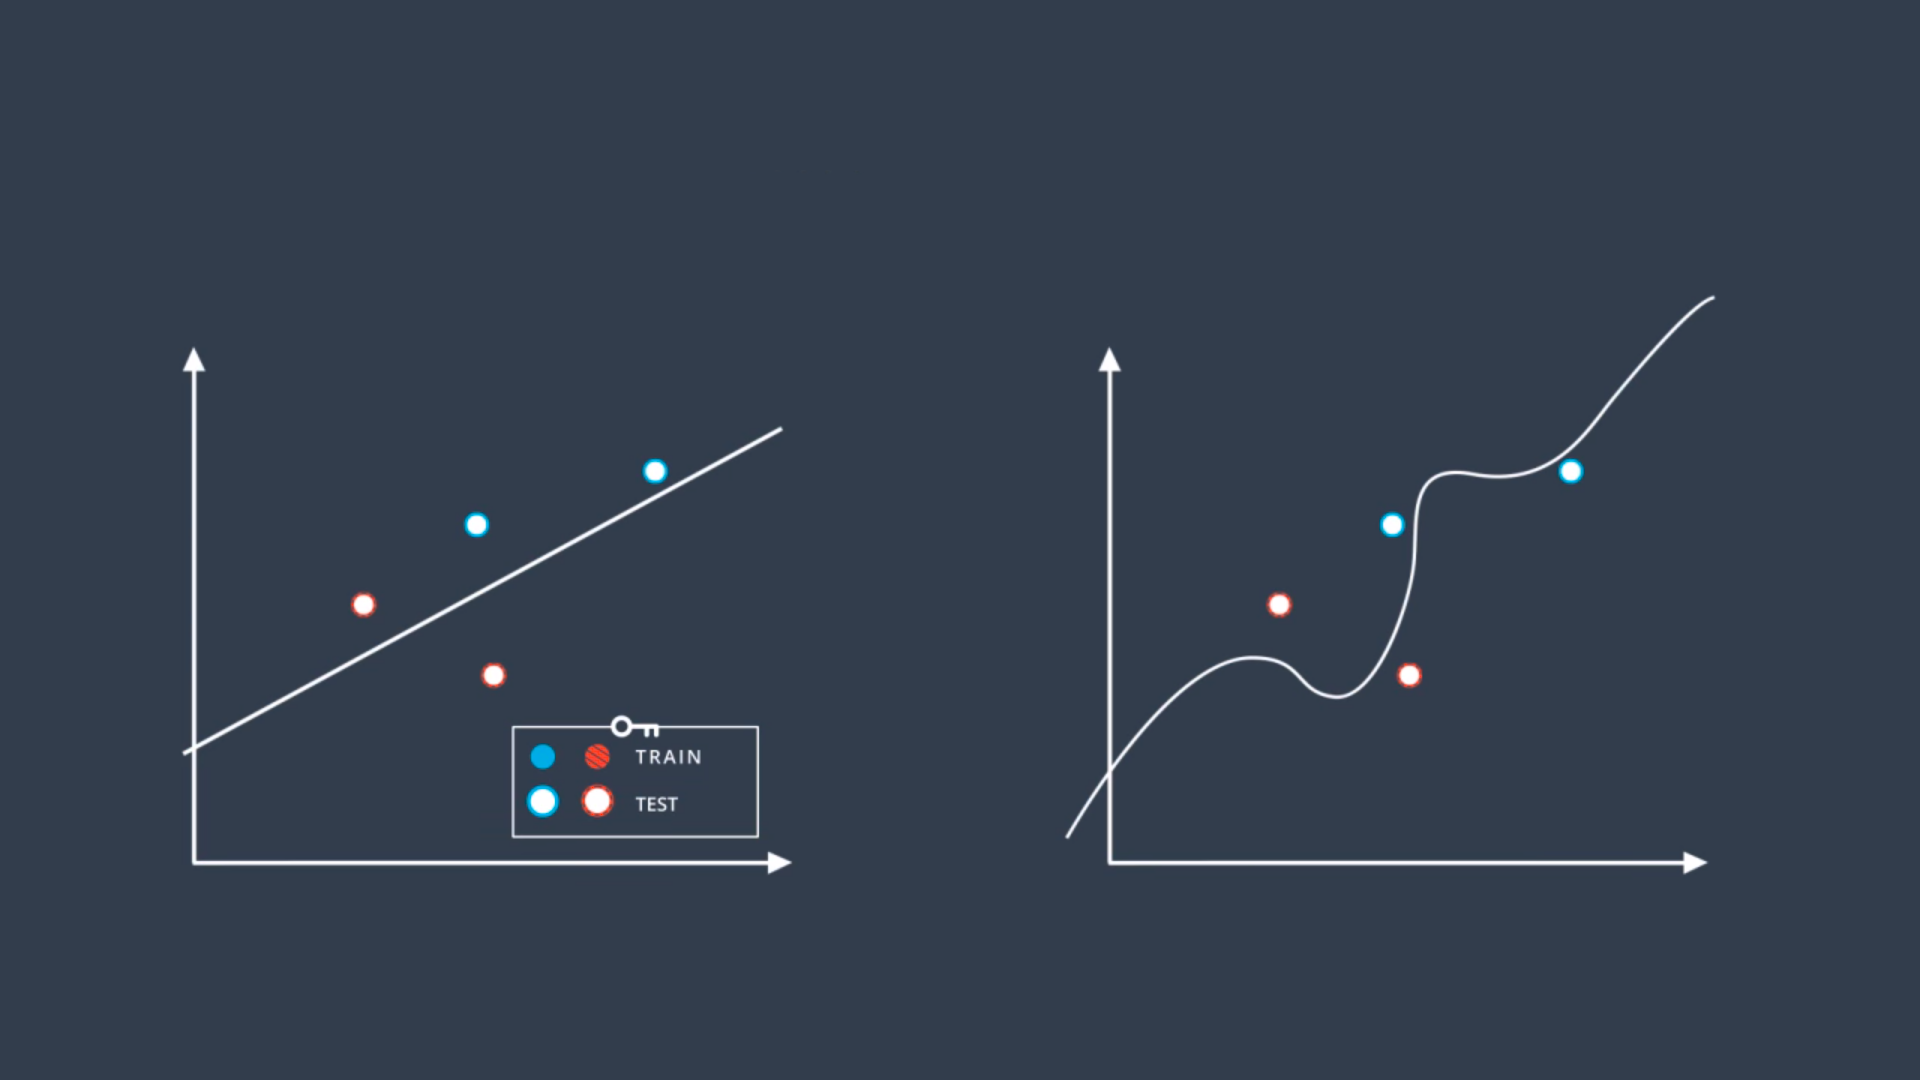
\includegraphics[width=1\paperwidth]{./overfitting4}}%
\frame{
	\frametitle{Overfitting problem}
	\framesubtitle{The importance of testing}
}
}


\frame{
	\frametitle{Overfitting and generalization}
\begin{itemize}

	\item \textbf{Underfitting} occurs when the model is not able to
	obtain a sufficiently low error value on the training set.
	\item \textbf{Overfitting} occurs when the gap between the training error and test error is too large.
	\item A model’s \textbf{capacity} is its ability to fit a wide variety of functions.
\end{itemize}
}


\frame{
	\frametitle{Regularization}
	\framesubtitle{Identify overfitting}
	
	\begin{figure}
		\centering
		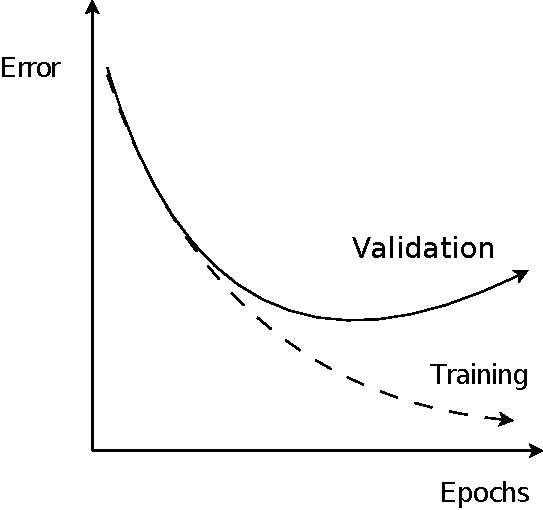
\includegraphics[height=0.7\textheight]{overf}
		\caption{Loss as epochs advance.}
		\label{fig:overf}
	\end{figure}
}


\section{Regularization}


\frame{
\frametitle{Regularization}

\begin{itemize}
	\item \textbf{Regularization} is any modification we make to a learning algorithm that is intended to reduce its generalization error but not its
	training error.
	
	\begin{itemize}
		\item Early termination
		\item L1, L2
		\item Dropout
	\end{itemize}
\end{itemize}

}


\frame{ 	
\frametitle{Regularization}
	\framesubtitle{Early termination}
	\begin{figure}
		\centering
		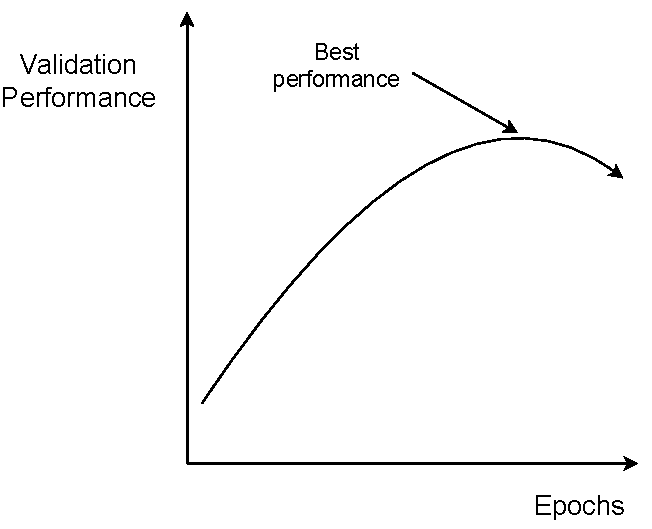
\includegraphics[height=0.7\textheight]{earlyt}
		\caption{Performance as epochs advance.}
		\label{fig:earlyt}
	\end{figure}
}


% --- Diapositiva 1: L2 Regularization ---
\begin{frame}{L2 Regularization (Weight Decay)}
	Adds a penalty equal to the square of the magnitude of coefficients.
	\vspace{0.3cm}
	\begin{columns}
		\begin{column}{0.5\textwidth}
			\textbf{The Math:}
			$$\mathcal{L}(W) = E(W) + \lambda \sum_{j=1}^{n} w_j^2$$
		\end{column}
		\begin{column}{0.5\textwidth}
			\textbf{Key Insights:}
			\begin{itemize}
				\item Penalizes large weights.
				\item Leads to \textbf{small, non-zero} weights.
			\end{itemize}
		\end{column}
	\end{columns}
\end{frame}

% --- Diapositiva 2: L1 Regularization ---
\begin{frame}{L1 Regularization (Lasso)}
	Adds a penalty equal to the absolute value of the magnitude of coefficients.
	\vspace{0.3cm}
	\begin{columns}
		\begin{column}{0.5\textwidth}
			\textbf{The Math:}
			$$\mathcal{L}(W) = E(W) + \lambda \sum_{j=1}^{n} |w_j|$$
		\end{column}
		\begin{column}{0.5\textwidth}
			\textbf{Key Insights:}
			\begin{itemize}
				\item Encourages \textbf{sparsity} (many weights become exactly zero).
				\item Useful for \textbf{feature selection}.
			\end{itemize}
		\end{column}
	\end{columns}
\end{frame}

% --- Diapositiva 3: Dropout ---
\begin{frame}{Dropout}
	A stochastic technique mainly used in Deep Learning.
	\vspace{0.3cm}
	\begin{itemize}
		\item \textbf{How it works:} During training, randomly "deactivate" a percentage $p$ of neurons in each forward pass \footnote{All neurons are used during inference, but weights are scaled by $p$.}.
		\item \textbf{Why it works:} 
		\begin{itemize}
			\item Prevents \textbf{co-adaptation} of neurons.
			\item Forces the network to learn redundant representations.
			\item Acts as an approximate model ensemble (averaging many sub-networks).
		\end{itemize}
	\end{itemize}
	\vspace{0.2cm}
	\centering
\end{frame}


\begin{frame}{Dropout}
	\centering
		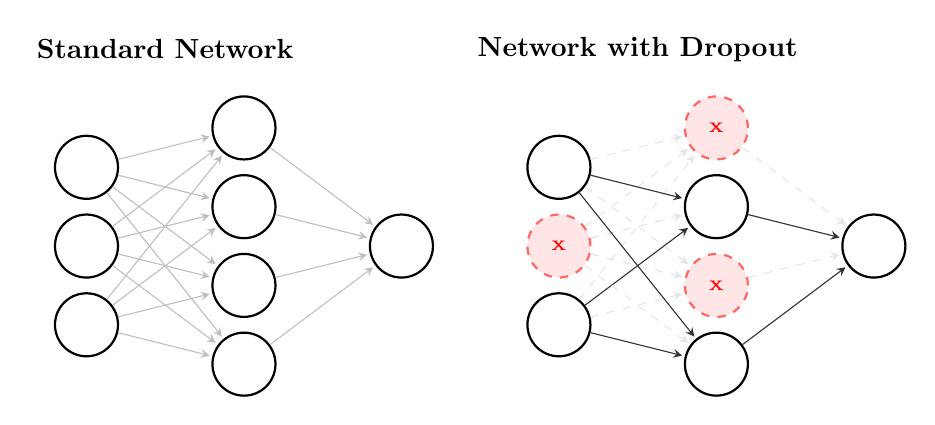
\begin{tikzpicture}[
			neuron/.style={circle, draw, minimum size=0.8cm, thick, fill=white},
			dropped/.style={circle, draw=red!60, minimum size=0.8cm, thick, fill=red!10, dashed},
			connection/.style={->, >=stealth, shorten >=1pt, gray!50},
			dropped_conn/.style={->, >=stealth, shorten >=1pt, gray!20, dashed}
			]
			
			% --- RED ESTÁNDAR (IZQUIERDA) ---
			\node[font=\bfseries] at (1, 4.5) {Standard Network};
			
			% Capa de Entrada
			\foreach \i in {1,2,3}
			\node[neuron] (in-\i) at (0, \i) {};
			% Capa Oculta
			\foreach \i in {1,2,3,4}
			\node[neuron] (h-\i) at (2, \i-0.5) {};
			% Capa de Salida
			\node[neuron] (out) at (4, 2) {};
			
			% Conexiones Estándar
			\foreach \i in {1,2,3}
			\foreach \j in {1,2,3,4}
			\draw[connection] (in-\i) -- (h-\j);
			
			\foreach \i in {1,2,3,4}
			\draw[connection] (h-\i) -- (out);
			
			
			% --- RED CON DROPOUT (DERECHA) ---
			\begin{scope}[xshift=6cm]
				\node[font=\bfseries] at (1, 4.5) {Network with Dropout};
				
				% Capa de Entrada
				\node[neuron] (din-1) at (0, 1) {};
				\node[dropped] (din-2) at (0, 2) {\color{red}\tiny \textbf{X}};
				\node[neuron] (din-3) at (0, 3) {};
				
				% Capa Oculta
				\node[neuron] (dh-1) at (2, 0.5) {};
				\node[dropped] (dh-2) at (2, 1.5) {\color{red}\tiny \textbf{X}};
				\node[neuron] (dh-3) at (2, 2.5) {};
				\node[dropped] (dh-4) at (2, 3.5) {\color{red}\tiny \textbf{X}};
				
				% Capa de Salida
				\node[neuron] (dout) at (4, 2) {};
				
				% Conexiones Activas y Desactivadas
				\foreach \i/\status in {1/active, 2/dropped, 3/active} {
					\foreach \j/\jstatus in {1/active, 2/dropped, 3/active, 4/dropped} {
						\ifnum\pdfstrcmp{\status}{active}=0
						\ifnum\pdfstrcmp{\jstatus}{active}=0
						\draw[connection, black!80] (din-\i) -- (dh-\j);
						\else
						\draw[dropped_conn] (din-\i) -- (dh-\j);
						\fi
						\else
						\draw[dropped_conn] (din-\i) -- (dh-\j);
						\fi
					}
				}
				
				\foreach \i/\status in {1/active, 2/dropped, 3/active, 4/dropped} {
					\ifnum\pdfstrcmp{\status}{active}=0
					\draw[connection, black!80] (dh-\i) -- (dout);
					\else
					\draw[dropped_conn] (dh-\i) -- (dout);
					\fi
				}
			\end{scope}
			
		\end{tikzpicture}
\end{frame}


\frame{
\frametitle{Model capacity selection}
\begin{figure}
	\centering
	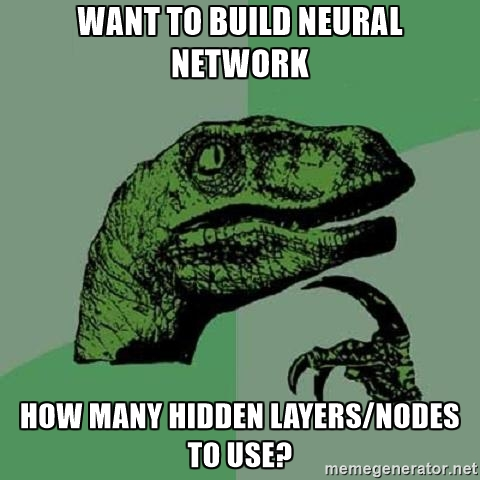
\includegraphics[height=0.7\textheight]{dl_meme3}
	\caption{Selecting depth}
	\label{fig:dlmeme3}
\end{figure}

}


\frame{
	\frametitle{Model capacity selection}
	\begin{itemize}
		\item Usually select the simplest model
		\item The optimal model is the one that has the same capacity than the problem.
		\begin{center}
			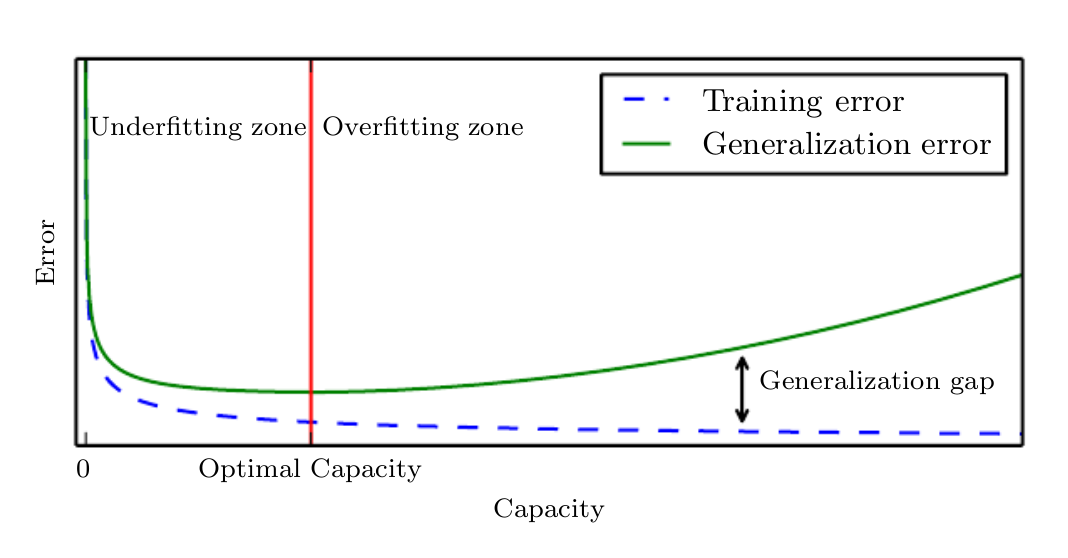
\includegraphics[width=0.8\linewidth]{capacity}
		\end{center}
	\end{itemize}
}


\frame{
\frametitle{Aditional information}
\begin{itemize}
	\item Chapter 5 Machine Learning Basics. Ian Goodfellow, et al. Deep Learning. MIT.
	\item Chapter 2 Training feed-forward neural networks. Buduma. Fundamentals of deep learning.
\end{itemize}
}



\frame{
\frametitle{References}
{\footnotesize
\begin{itemize}
   \item [Goodfellow] Goodfellow, I., Bengio, Y., Courville, A., \& Bengio, Y. (2016). Deep learning (Vol. 1). Cambridge: MIT press.
   \item [Sucar15] Sucar, Luis Enrique. Probabilistic Graphical Models: Principles and Applications. Springer, 2015.
   \item [Smola] Alex Smola and S.V.N. Vishwanathan, Introduction to Machine Learning, Cambirdge University Press.
   \item [Udacity] Self Driving Car Nanodegree
   \item [Srivastava] Srivastava, N., Hinton, G., Krizhevsky, A., Sutskever, I., \& Salakhutdinov, R. (2014). Dropout: a simple way to prevent neural networks from overfitting. The Journal of Machine Learning Research, 15(1), 1929-1958.
   \item [HJC] https://houstonjobconnection.com/article/what-is-a-dataset-in-machine-learning
\end{itemize}
}
}


\end{document}